\section{Dataset and Preprocessing}
\label{sec:dataset}

\subsection{Data Source}
\label{sec:data_source}
The dataset originates from the DaT-SPECT Parkinson's Disease Classification challenge, comprising \textbf{1,363 NIfTI scans} from \textbf{15 unique scanner sites}. Binary labels indicate pathological (dopaminergic deficit) vs. normal scans. The class distribution is 54.8\% positive (747 scans) and 45.2\% negative (616 scans). One scan failed quality control during preprocessing, yielding 1,362 usable scans.

\subsection{Scanner Heterogeneity Analysis}
\label{sec:heterogeneity}
Figure~\ref{fig:voxel_dist} (reproduced from our analysis) summarizes the substantial heterogeneity:

\begin{figure}[htbp]
    \centering
    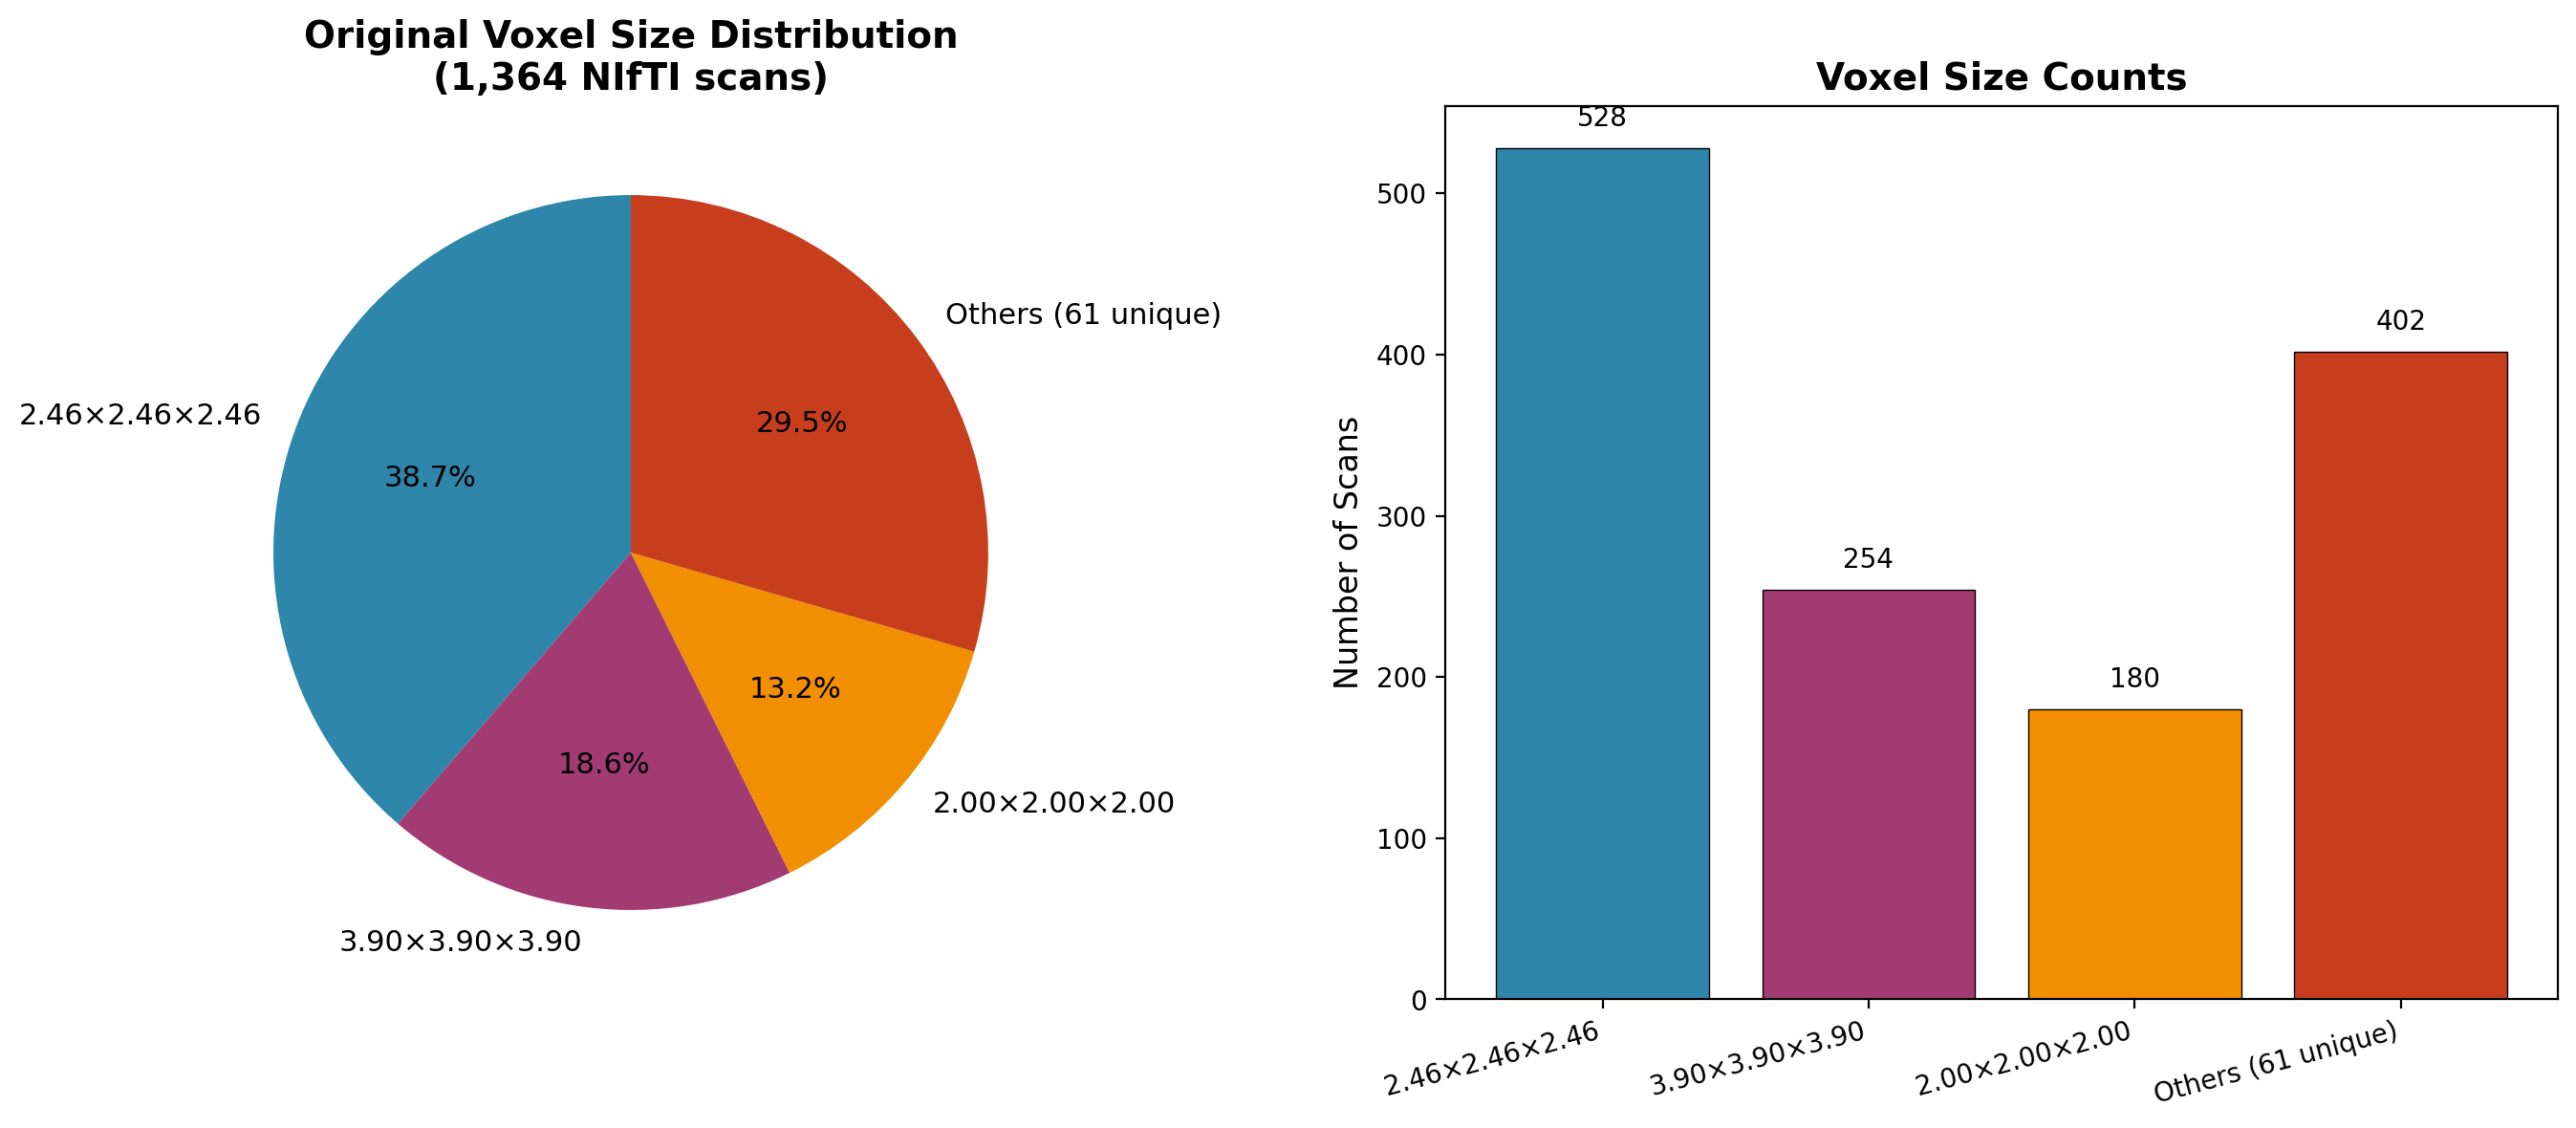
\includegraphics[width=0.9\linewidth]{figures/voxel_distribution.png}
    \caption{Original voxel size distribution across 1,364 NIfTI scans. (Left) Pie chart showing percentage of scans per voxel size. (Right) Bar chart with counts. Dominant resolutions are 2.46~mm (38.8\%, 528 scans) and 3.90~mm (18.6\%, 254 scans); 64 unique voxel sizes total.}
    \label{fig:voxel_dist}
\end{figure}

\begin{table}[htbp]
\centering
\caption{Top voxel sizes in raw dataset (1,363 scans).}
\label{tab:voxel_sizes}
\begin{tabular}{lccc}
\toprule
\textbf{Voxel Size (mm)} & \textbf{Count} & \textbf{Percentage} & \textbf{Typical Shape} \\
\midrule
2.46 $\times$ 2.46 $\times$ 2.46 & 528 & 38.8\% & 256$\times$256$\times$256, 128$\times$128$\times$128 \\
3.90 $\times$ 3.90 $\times$ 3.90 & 254 & 18.6\% & 128$\times$128$\times$128, 128$\times$128$\times$87 \\
2.30 $\times$ 2.30 $\times$ 2.30 & 130 & 9.5\% & 134$\times$134$\times$112 \\
2.40 $\times$ 2.40 $\times$ 2.40 & 110 & 8.1\% & 144$\times$144$\times$112 \\
Others (60 unique) & 341 & 25.0\% & Various \\
\midrule
\textbf{Total} & \textbf{1,363} & \textbf{100\%} & \textbf{66 unique shapes} \\
\bottomrule
\end{tabular}
\end{table}

The physical field of view varies from 96~mm to 284~mm across dimensions, necessitating a unified preprocessing pipeline.

\subsection{Preprocessing Pipeline}
\label{sec:preprocessing}
All scans undergo identical deterministic preprocessing:

\begin{enumerate}
    \item \textbf{RAS Reorientation:} NIfTI affine matrices are used to reorient volumes to Right-Anterior-Superior (RAS) coordinate system using nibabel's orientation transforms.
    \item \textbf{Isotropic Resampling:} Volumes are resampled to 2.0~mm isotropic voxels via trilinear interpolation. Scaling factor per dimension: $f_i = \frac{\text{voxel}_i}{2.0}$.
    \item \textbf{Center-of-Mass Alignment:} The center-of-mass (COM) of thresholded intensities ($>$5th percentile) is computed and translated to the center of an 80$^3$ grid (center = 39.5). Affine transform: $\mathbf{T}(\mathbf{x}) = \mathbf{x} - \text{COM} + \mathbf{C}$.
    \item \textbf{Full Volume Retention:} The entire 80$\times$80$\times$80 grid is retained (no cropping) because striatal signal spans the full field-of-view in some acquisitions.
    \item \textbf{Per-Volume Z-Score Normalization:} Each volume is normalized independently: $\tilde{v} = \frac{v - \mu_v}{\sigma_v + 10^{-8}}$, where $\mu_v, \sigma_v$ are computed per-volume. This prevents dataset-level statistics from leaking into validation folds.
    \item \textbf{Inference Normalization:} At inference, intensities are clipped to [1st, 99th] percentile and min-max scaled to [0, 1].
\end{enumerate}

Figure~\ref{fig:preprocessing} illustrates the before/after transformation.

\begin{figure}[htbp]
    \centering
    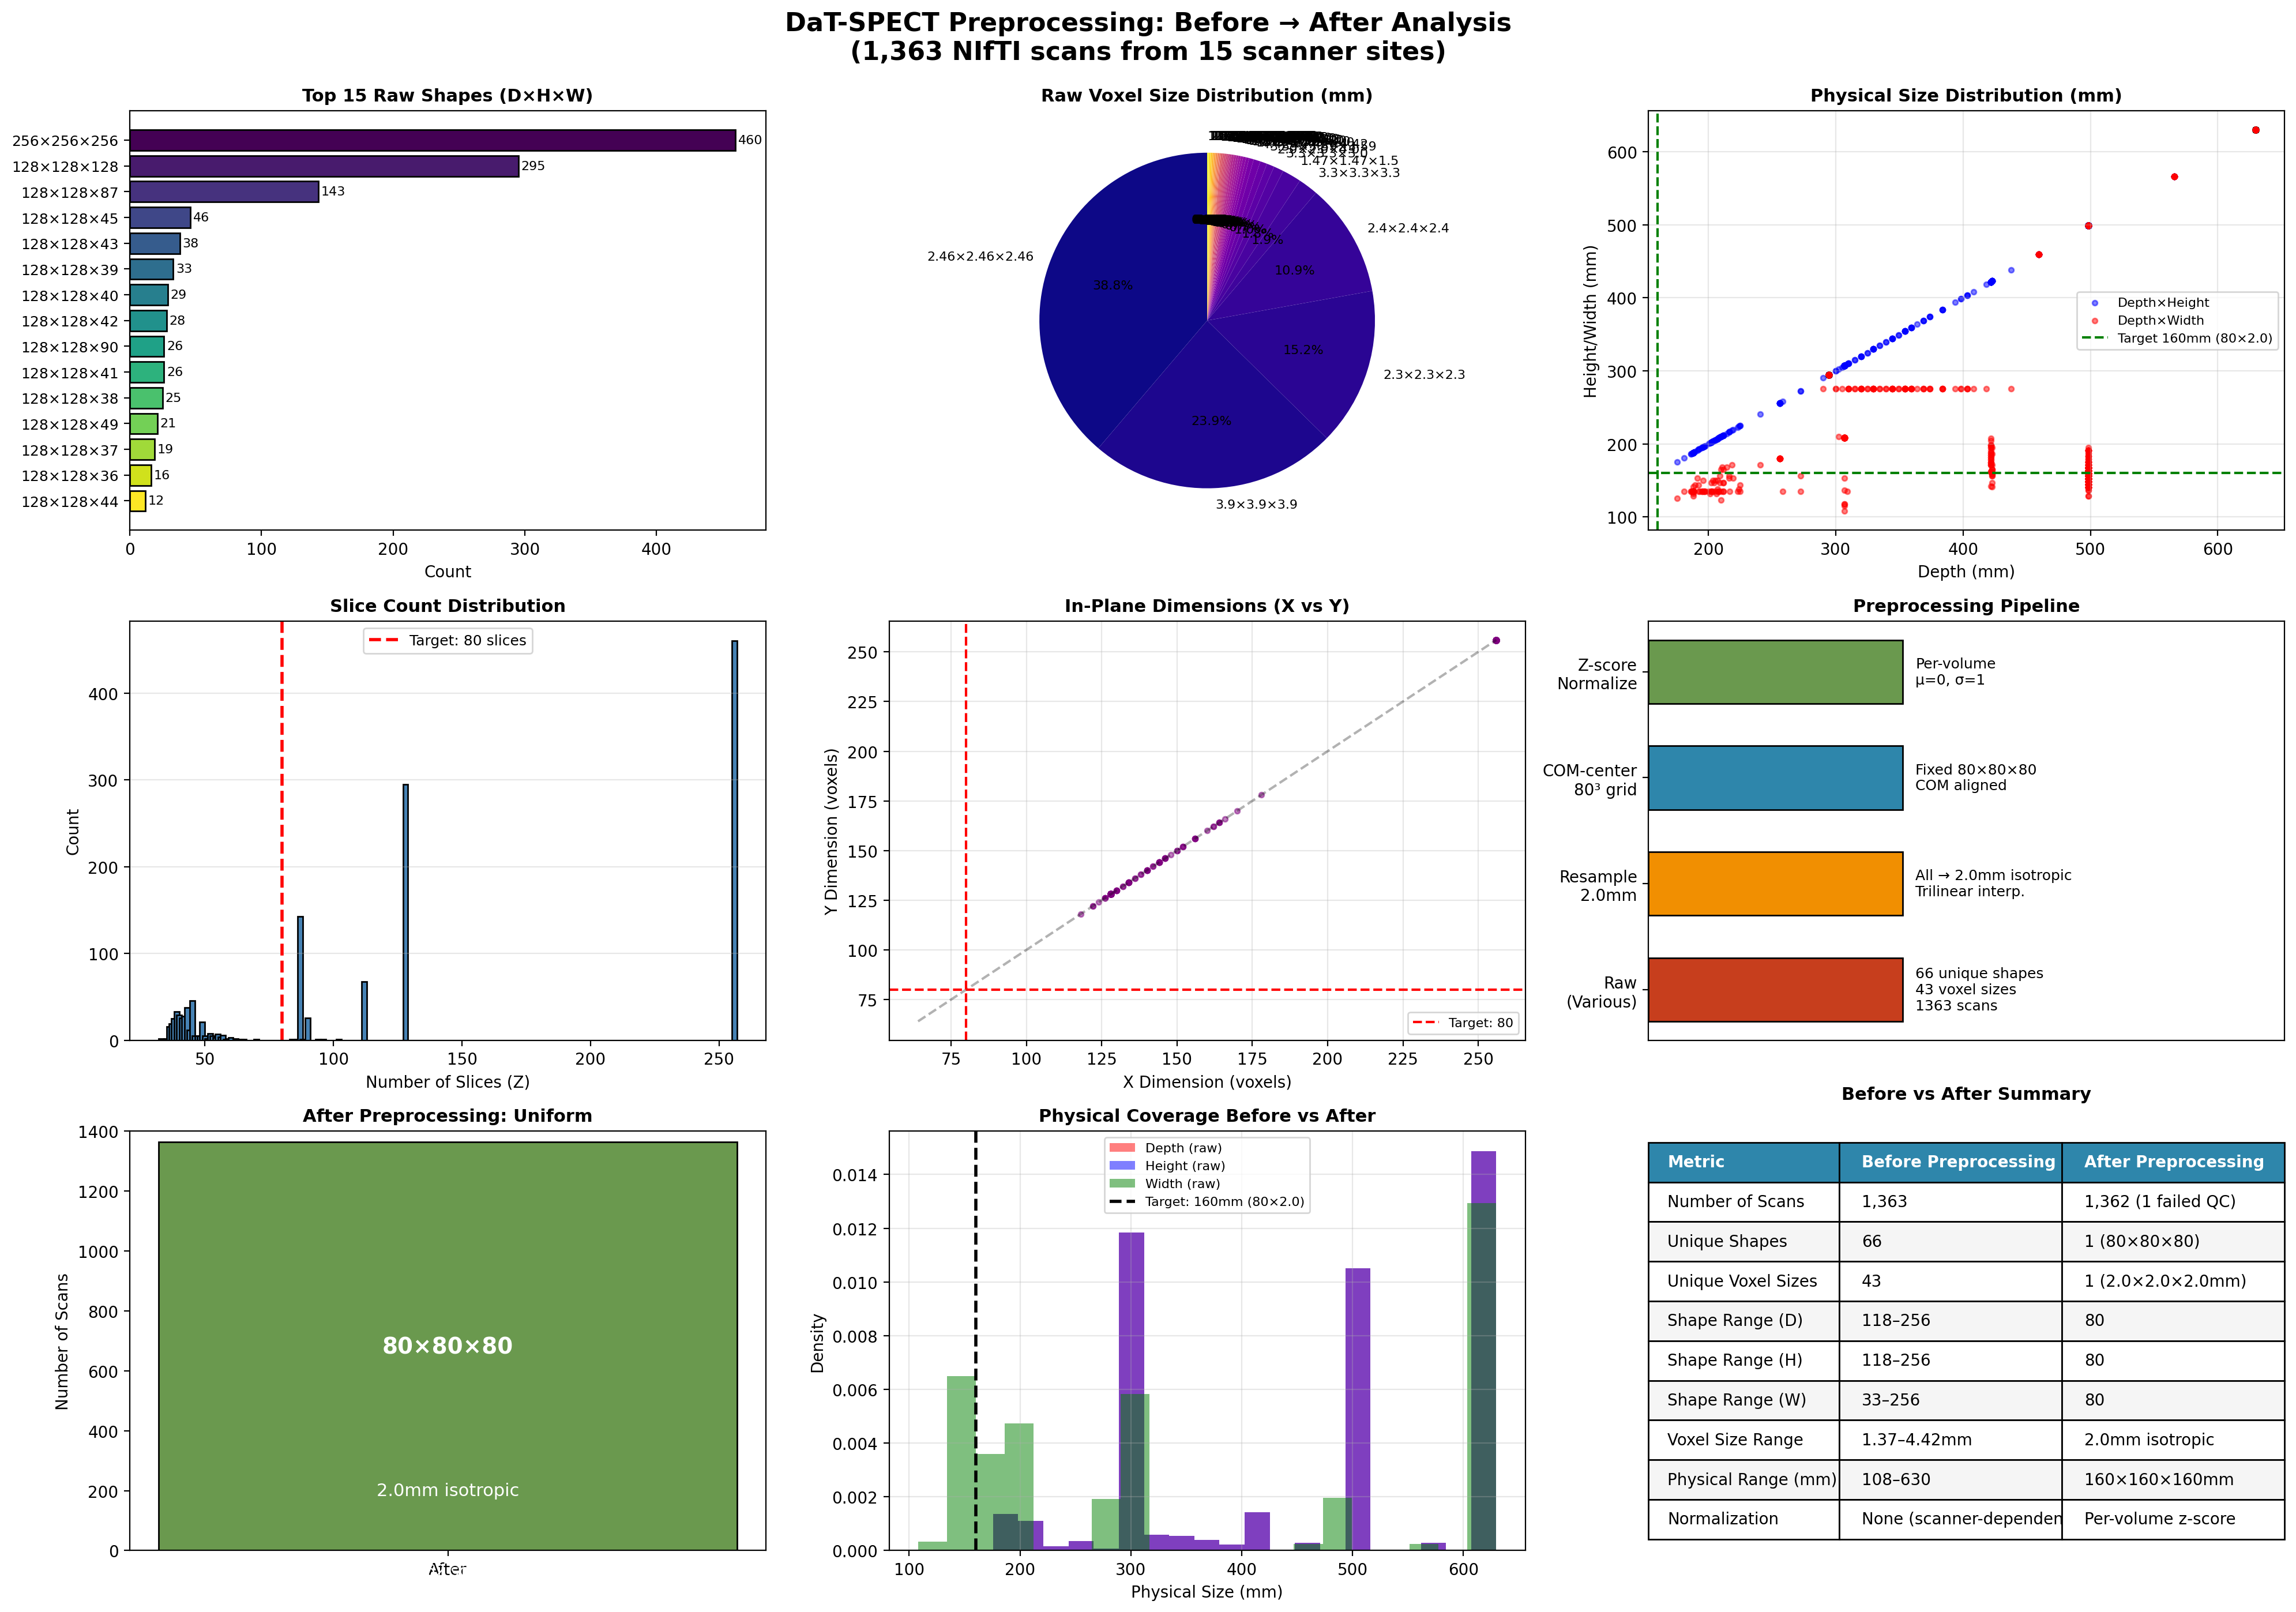
\includegraphics[width=0.95\linewidth]{figures/preprocessing_before_after.png}
    \caption{Before/after preprocessing analysis. (Top row) Raw data diversity: 66 unique shapes, 66 voxel sizes, physical coverage 96--284~mm. (Middle) Pipeline stages. (Bottom) Uniform 80$^3$ output at 2.0~mm isotropic with summary statistics table.}
    \label{fig:preprocessing}
\end{figure}

\begin{table}[htbp]
\centering
\caption{Preprocessing summary: before vs. after.}
\label{tab:preprocessing_summary}
\begin{tabular}{lll}
\toprule
\textbf{Metric} & \textbf{Before} & \textbf{After} \\
\midrule
Scans & 1,363 & 1,362 (1 failed QC) \\
Unique shapes & 66 & 1 (80$\times$80$\times$80) \\
Unique voxel sizes & 66 & 1 (2.0~mm isotropic) \\
Shape range (D/H/W) & 126--256 / 36--128 & 80 / 80 / 80 \\
Voxel size range & 1.47--3.90~mm & 2.0~mm \\
Physical coverage & 96--284~mm & 160$\times$160$\times$160~mm \\
Normalization & Scanner-dependent & Per-volume z-score \\
\bottomrule
\end{tabular}
\end{table}

\subsection{Atlas-Based Template}
\label{sec:atlas}
An atlas template is constructed by averaging all preprocessed training volumes. This template serves as the reference for normalized cross-correlation (NCC) alignment during inference (Section~\ref{sec:inference}). The template captures the average striatal anatomy across the population, enabling robust registration without external atlases.

\subsection{Scanner Groups for Cross-Validation}
\label{sec:groups}
The 15 scanner sites (derived from site metadata) serve as grouping variables for cross-validation. Distribution: 8 sites with $\ge$100 scans, 4 sites with 50--100, 3 sites with $<$50. This ensures each fold contains a representative mix of acquisition protocols.